\section{Каркас III}
\subsection{Условие задания}
Дан взвешенный неориентированный граф из $N$ вершин и $M$ ребер.
Требуется найти в нем каркас минимального веса. (Алгоритм Прима)

\subsection{Примеры исходного кода}
Для нахождения каркаса минимального веса взвешенного неориентированного
графа был создан метод \mitext{mst()} (\textit{Minimal Spanning Tree}):
\begin{minted}{typescript}
mst(): Graph {
  if (!this.weighted || this.oriented) {
    throw new GraphNotWeightedUnoriented()
  }

  const mst = new Graph(true, false) // минимальное остовное дерево
  const visited = new Set<string>() // множество посещенных вершин

  // взять любую вершину как начальную (здесь первая)
  const startVertex = this.adj.keys().next().value
  if (!startVertex) {
    throw new GraphIsEmpty()
  }
  visited.add(startVertex)
  mst.addNode(startVertex)

  while (visited.size < this.adj.size) { // пока не посетим все вершины
    // ребра, которые соединяют посещенные вершины с непосещенными
    const edges: Array<Edge> = []

    for (const vertex of visited) { // найти такие ребра
      for (const [neighbor, weight] of this.adj.get(vertex)!) {
        if (!visited.has(neighbor)) {
          edges.push({from: vertex, to: neighbor, weight});
        }
      }
    }

    if (edges.length === 0) {
      // Не все вершины еще посещены, но мы не смогли найти новые ребра.
      // Это значит, что граф несвязный.
      throw new GraphIsNotConnected()
    }

    // выбрать ребро с наименьшим весом
    edges.sort((a, b) => a.weight - b.weight)
    const {from, to, weight} = edges[0]

    // добавить ребро в минимальное остовное дерево
    mst.addNode(to)
    mst.connect(from, to, weight)
    visited.add(to)
  }

  return mst
}
\end{minted}

\subsection{Краткое описание алгоритма}
Основная идея заключается в том, чтобы начать с одной вершины и пошагово добавлять ребра
минимального веса, соединяющие посещенные вершины с непосещенными.

Создается новый граф \mitext{mst}, представляющий минимальное остовное дерево.
Также создается множество \mitext{visited} для отслеживания посещенных вершин.
Выбирается любая вершина в качестве начальной. В данной реализации используется
первая вершина из списка вершин графа.

Пока не посещены все вершины графа, выполняется цикл:
\begin{enumerate}
  \item Создается массив \mitext{edges}, содержащий ребра, соединяющие посещенные вершины с непосещенными.
  \item Если массив \mitext{edges} пуст, это означает, что граф несвязный (ошибка).
  \item Ребра в массиве сортируются по весу, и выбирается ребро с минимальным весом.
  \item Выбранное ребро добавляется в остовное дерево, связывая вершины \mitext{from} и \mitext{to} с весом
  \mitext{weight}. Вершина \mitext{to} помечается как посещенная.
\end{enumerate}

\subsection{Примеры входных и выходных данных}
\subsubsection{Входные данные}
\begin{figure}[H]
  \begin{minipage}{0.5\textwidth}
    \centering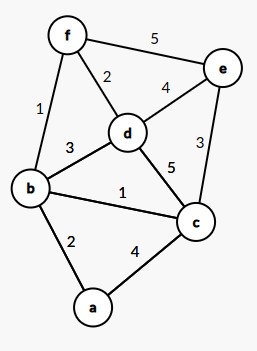
\includegraphics[width=0.6\linewidth]{figs/task-7/graph-7.png}
  \end{minipage}
  \begin{minipage}{0.5\textwidth}
    \centering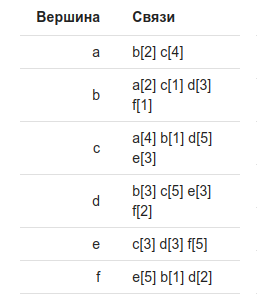
\includegraphics[width=0.6\linewidth]{figs/task-7/adj-7.png}
  \end{minipage}
  \caption{Неориентированный взвешенный граф}
\end{figure}

\begin{minted}{js}
{
  "weighted": true,
  "oriented": false,
  "adj": {
    "a": {
      "b": 2,
      "c": 4
    },
    "b": {
      "a": 2,
      "c": 1,
      "d": 3,
      "f": 1
    },
    "c": {
      "a": 4,
      "b": 1,
      "d": 5,
      "e": 3
    },
    "d": {
      "b": 3,
      "c": 5,
      "e": 3,
      "f": 2
    },
    "e": {
      "c": 3,
      "d": 4,
      "f": 5
    },
    "f": {
      "e": 5,
      "b": 1,
      "d": 2
    }
  }
}
\end{minted}

\subsubsection{Выходные данные}
\begin{figure}[H]
  \begin{minipage}{0.5\textwidth}
    \centering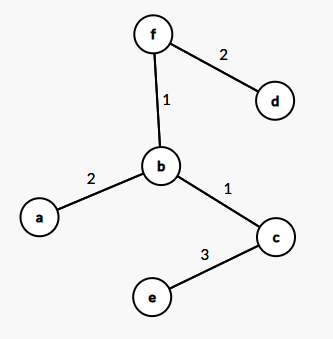
\includegraphics[width=0.8\linewidth]{figs/task-7/res-graph-7.png}
  \end{minipage}
  \begin{minipage}{0.5\textwidth}
    \centering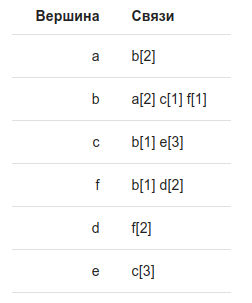
\includegraphics[width=0.6\linewidth]{figs/task-7/res-7.png}
  \end{minipage}
  \caption{Результат работы}
\end{figure}